\documentclass[12pt, letterpaper]{article}
\usepackage[english]{babel}
\usepackage{graphicx}
\usepackage{float}
\usepackage{hyperref}

\title{DAT510 - Assignment 2}
\author{Fr\o ydis J\o rgensen}

\begin{document}
\begin{titlepage}
\maketitle
\end{titlepage}

\begin{abstract}
Throughout this assignment, I have created a simplified real-world application to demonstrate how we use the Diffie-Hellman key exchange scheme to create a secret key between Alice and Bob. Then I have strengthened the key by using the pseudo-random number generator Blum Blum Shub and used resources from Assignment 1 to encrypt and decrypt the messages between Alice and Bob. Part 1 is a staged scenario where I go into detail about how the different steps work. Part 2 uses the functions from Part 1 to create secure communication from one server to another.
\end{abstract}

\section*{Introduction}
In this project, I will implement and show how the Diffie-Hellman key exchange scheme and the pseudo-random number generator Blum Blum Shub works.  I do also use my Simple DES (SDES) from the previous assignment for encrypting and decrypting but will not talk about how SDES works in this assignment. The goal is to use these parts to create a secure communication scenario between Alice in Bob.

\section*{Design and Implementation}
\subsection*{Part 1}
The first part of this assignment required making a secure communication scenario by following 8 steps.
The first step is to decide on some global parameters for a Diffie-Hellman-like key exchange. So Alice and Bob agree on a cyclic group of order p which had to be a prime as 2q +1. This is a so-called safe prime and we get it if we take a Sophie Germain prime as q, and we get a new prime. So in this case I used Sophie Germain prime 359. 2*359 + 1 = 719. So the shared prime number between Alice and Bob is 719. We can therefore say that the cyclic group is Z*719, which means that after the operations, done by Diffie-Hellmann key exchange, we will end up with a number between g = 2, which was predefined as the generator, and p = 719. Figure \ref{fig:step1} shows the start at my main function where the generator g and the shared prime is defined.

\begin{figure}[H]
  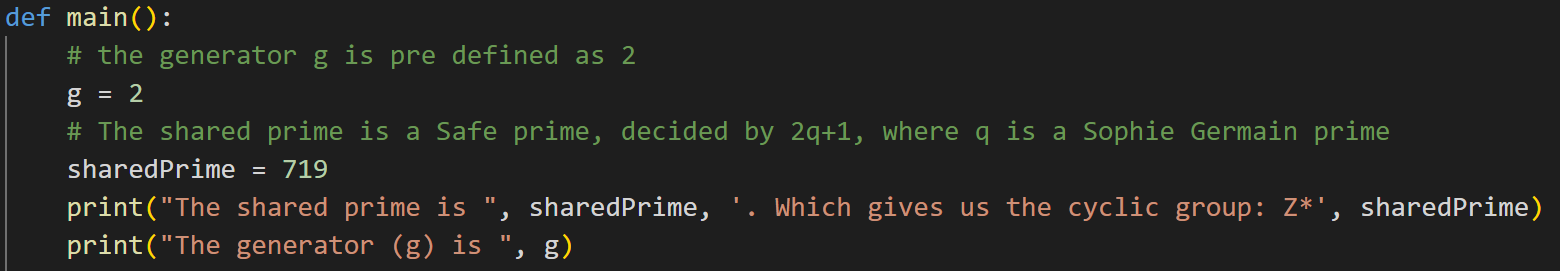
\includegraphics[width=\linewidth]{code_snippets/step1.PNG}
  \caption{Start of my main function, defined g and the shared prime}
  \label{fig:step1}
\end{figure}

The second step is to follow the Diffie-Hellman's key exchange scheme and create Alice's and Bob's key pair. For their private key, I just chose a random number, so Alice's private key is 217, and Bob's private key is 131. The only requirements for the private keys are that they are smaller than their shared prime and a positive natural number. To create the public key from the private key I created a method, which is shown in Figure \ref{fig:step2_func}. To create the public key, the function does this operation: $$g^{privateKey}\ mod\ sharedPrime$$

\begin{figure}[H]
  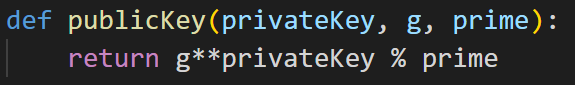
\includegraphics[width=300px]{code_snippets/step2_func.PNG}\centering
  \caption{The function to create the public key}
  \label{fig:step2_func}
\end{figure}

Figure \ref{fig:step2} shows how the private and public key are defined for Alice and Bob.

\begin{figure}[H]
  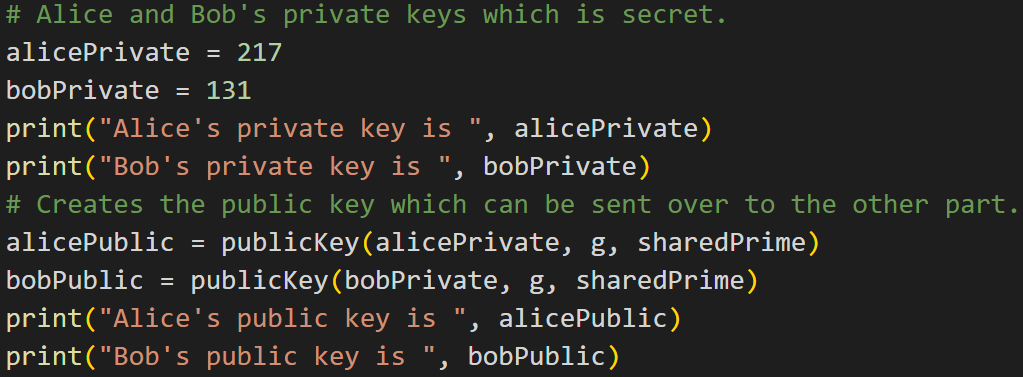
\includegraphics[width=\linewidth]{code_snippets/step2.PNG}
  \caption{Defines private key and calls a function to create the public key}
  \label{fig:step2}
\end{figure}

The third step is to send the public key to the part you want to connect with. Since this is a staged scenario and both Alice and Bob run on the same program this is not necessary. But we will take a closer look at this step in part 2. 

The fourth step is to create a shared key. The shared key is created as shown in Figure \ref{fig:step4_func} by doing this operation: $$publickey^{privateKey} \ mod \ sharedPrime$$

\begin{figure}[H]
  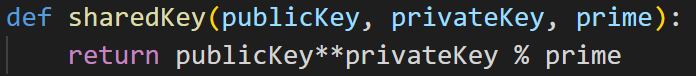
\includegraphics[width=300px]{code_snippets/step4_func.PNG}\centering
  \caption{The function to create the shared secret key}
  \label{fig:step4_func}
\end{figure}

Both Alice and Bob should now have the same shared key, which is a secret and should not be shared with anyone else. As shown in Figure \ref{fig:step4}, I check that the shared keys are the same for both Alice and Bob. If they do not have the same number something wrong happened along the way and they do not have a connection.

\begin{figure}[H]
  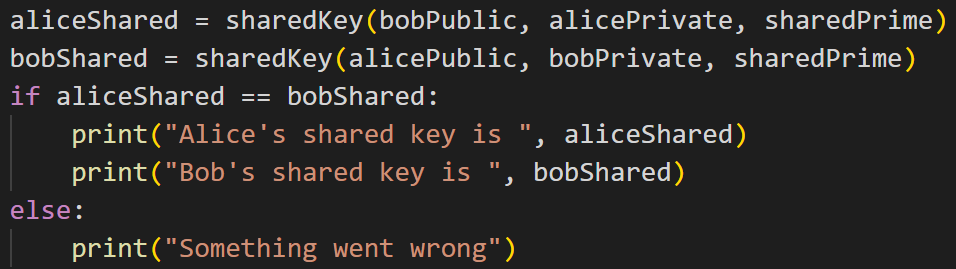
\includegraphics[width=\linewidth]{code_snippets/step4.PNG}
  \caption{Calls the function to get the shared key, and check if Alice and Bob have the same key}
  \label{fig:step4}
\end{figure}

At this point, we are done with the Diffie-Hellman's key exchange, but since Alice and Bob are concerned about the strength of the shared key, they want to use a cryptographically strong pseudo-random number generator (CSPRNG). I choose to use a pseudo-random number generator named Blum Blum Shub (BBS) in this fifth step. Blum Blum Shub takes the form: $$x_{n+1} = x^{2}_{n} \ mod \ M$$
$x_{0}$ is called the seed, which in this case is the shared secret key. M is p*q where both q and p is a prime number and both are congruent to 3 mod 4. Both 7 and 11 fulfills that, and therefore I chose my M to be 7*11 = 77. This method is based on taking the least significant bit for each operation, as shown in Figure \ref{fig:step5}. On the way, we have to check that the seed we start with or the new seeds that we create not are 0 or 1. We do also have to check that the seed values do not share factors with either p or q Ref \cite{BBS}.

\begin{figure}[H]
  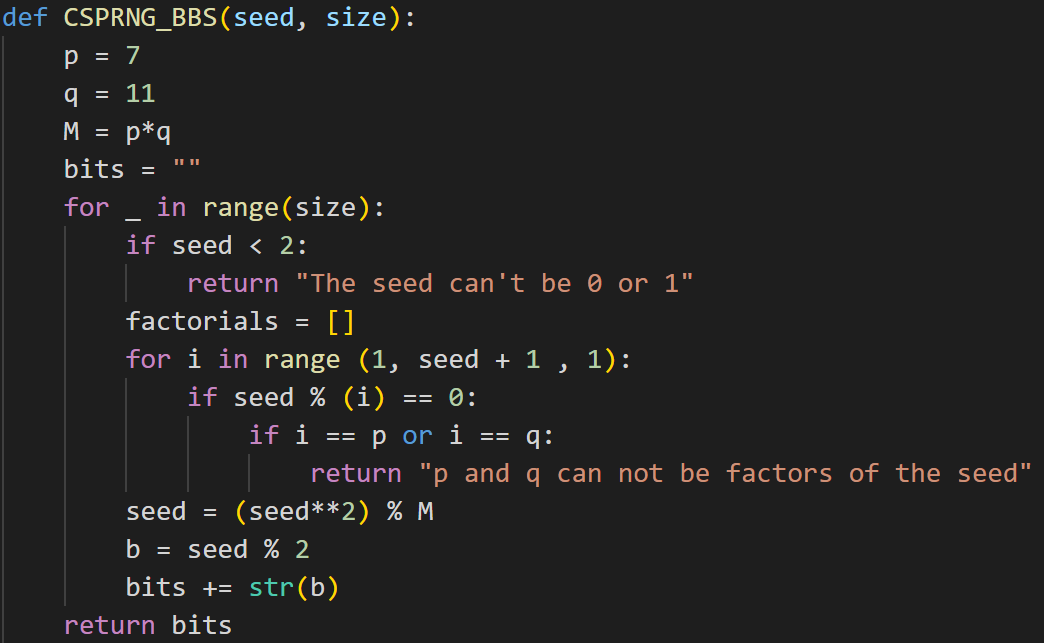
\includegraphics[width=\linewidth]{code_snippets/step5.PNG}
  \caption{The function that performs Blum Blum Shub}
  \label{fig:step5}
\end{figure}

As shown in Figure \ref{fig:step6} we use the CSPRNG and creates a secret key which is of length 10 bits, but I convert it into a decimal. The reason why I chose a bit length of 10 is that In the next step we are going to encrypt a text and send it to Bob. For the encryption, I chose to use SDES from the previous assignment. This is not secure encryption, but since the encryption is not the focus in this assignment I used SDES instead of importing something more secure. SDES encryption takes in a 10-bit long key and encrypts 8-bit blocks at a time. As shown in Figure \ref{fig:step6} you get the choice of writing your own message or using a predefined message. I convert the message into bits and split it up in 8-bit blocks. Then the program goes through the list of the 8-bit blocks and encrypts them using our 10-bit key.

\begin{figure}[H]
  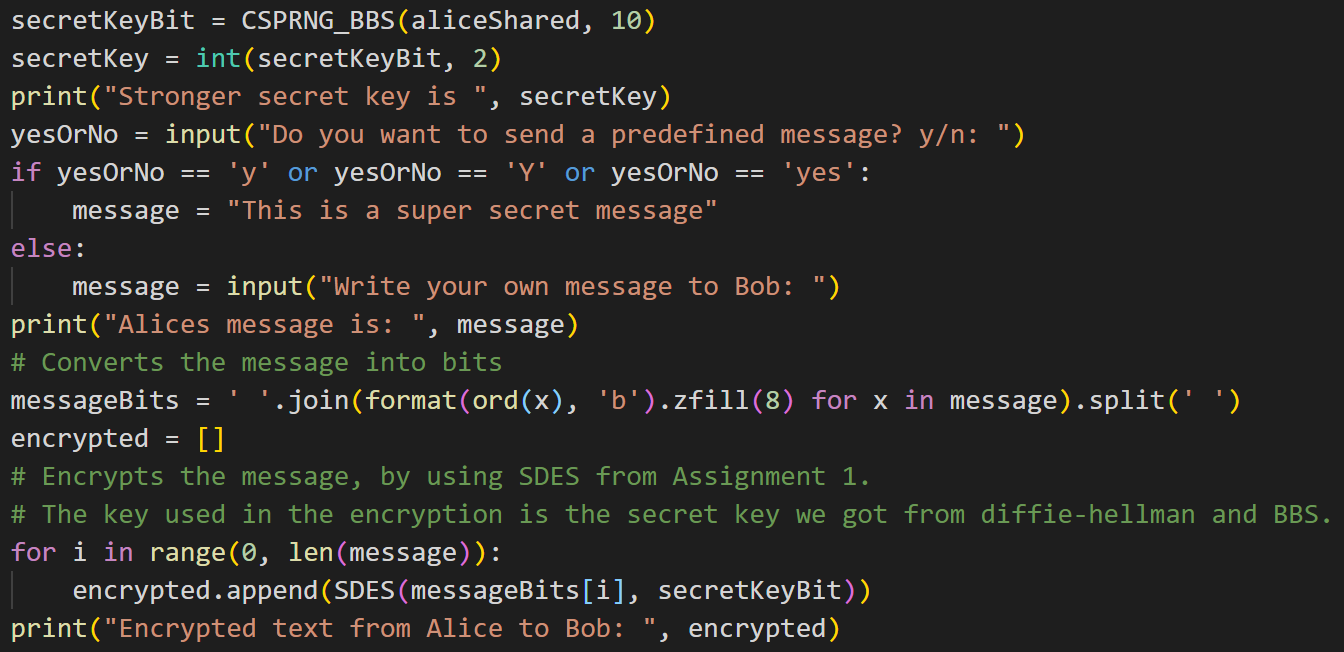
\includegraphics[width=\linewidth]{code_snippets/step6.PNG}
  \caption{Calls Blum Blum Shub and SDES to secure the key and encrypt a text}
  \label{fig:step6}
\end{figure}

The next step is for Bob to decrypt the message from Alice. At this point, we already know that Alice and Bob got the same shared key and used the same BBS. So as shown in Figure \ref{fig:step7}, we take in 8-bit blocks from the cipher and decrypt it using the same key, which will give us the message from Alice in plaintext.

\begin{figure}[H]
  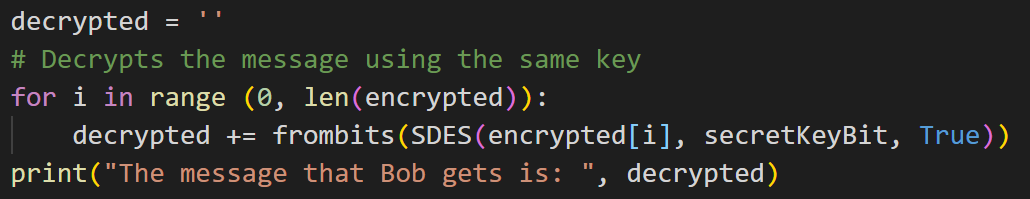
\includegraphics[width=\linewidth]{code_snippets/step7.PNG}
  \caption{Calles SDES to decrypt the cipher from Alice}
  \label{fig:step7}
\end{figure}

I have now shown a secure communication scenario between Alice and Bob. If someone else would have gotten the cipher, they could not have deciphered it, because the key was created from both Alice's private key and Bob's private key and their shared prime, which is a secret. 

\subsection*{Part 2}
The second part of this assignment is to connect Alice's and Bob's servers and generate a shared secret key and then send messages to each other in a secure way. Since we do this on localhost I needed to run the localhosts on two different ports. Therefore, Alice's localhost is running on port 3000, and Bob's on port 5000. To run these I use both bash and PowerShell so that they don't overwrite each other. Alice's and Bob's servers are very similar. They have the same pages and functions. The main difference is that they have different defined private keys, and therefore different public keys, but they have the same Prime and generator. For simplicity, I have used the same numbers as in Part 1. The first page you get to when you have started the localhost's http://127.0.0.1:3000 and http://127.0.0.1:5000 returns a text with an URL to /getPub, if you want to create a secure connection with the other server. 
\\
When Bob directs to /getPub the code as shown in Figure \ref{fig:getPub} will be executed. This starts off by fetching Alice's public key, which he gets from Alice's server at /sendPub, as shown in Figure \ref{fig:sendPub}, which uses the function shown in Figure \ref{fig:step2_func}. If Bob gets a response from Alice's server he uses the sharedKey function which is shown in Figure \ref{fig:step4_func} and then the Blum Blum Shub function which is shown in Figure \ref{fig:step5}. This creates the secret key and he now has the key to encrypt messages to Alice. The page returns a text saying that he has a secure connection with Alice and a link to /sendMsg if he wants to send Alice a message.

\begin{figure}[H]
  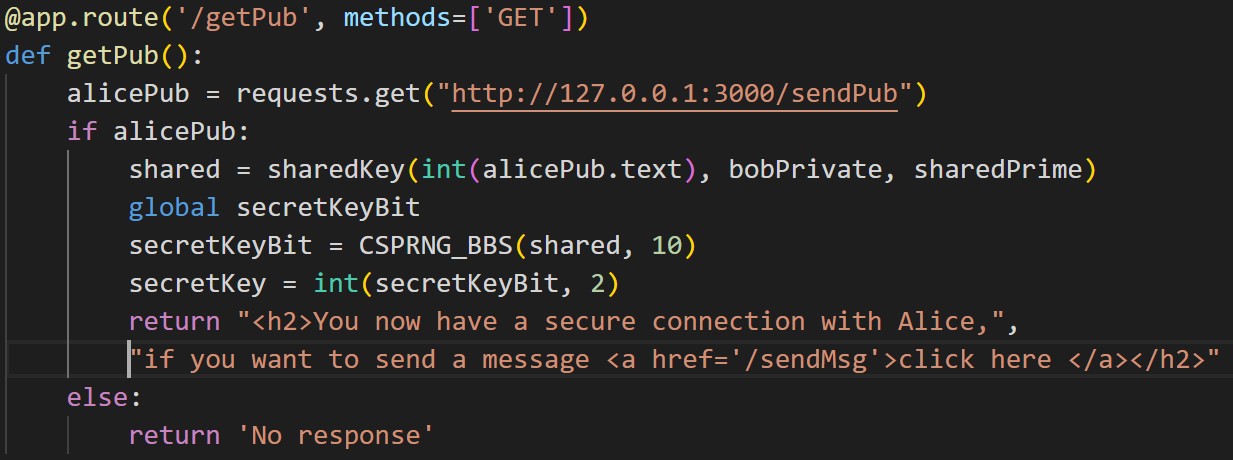
\includegraphics[width=\linewidth]{code_snippets/getPub.PNG}
  \caption{Bob's server: Fetches Alices public key and creates the shared secret key}
  \label{fig:getPub}
\end{figure}

\begin{figure}[H]
  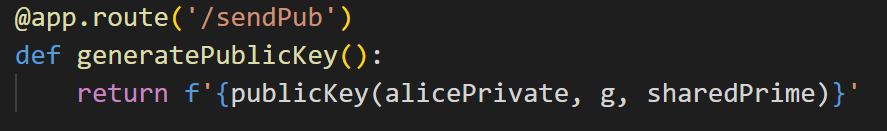
\includegraphics[width=\linewidth]{code_snippets/sendPub.PNG}
  \caption{Alice's server: creates Alice's public key and returns it}
  \label{fig:sendPub}
\end{figure}

If Bob goes to /sendMsg before he has established a secure connection with Alice, he will be told that he first has to go to /getPub before he can send a message. If the secure connection has been established a simple template as shown in Figure \ref{fig:temp}, which gives an input field to write a message and a submit button. I have used Bootstrap to make the page a bit prettier.

\begin{figure}[H]
  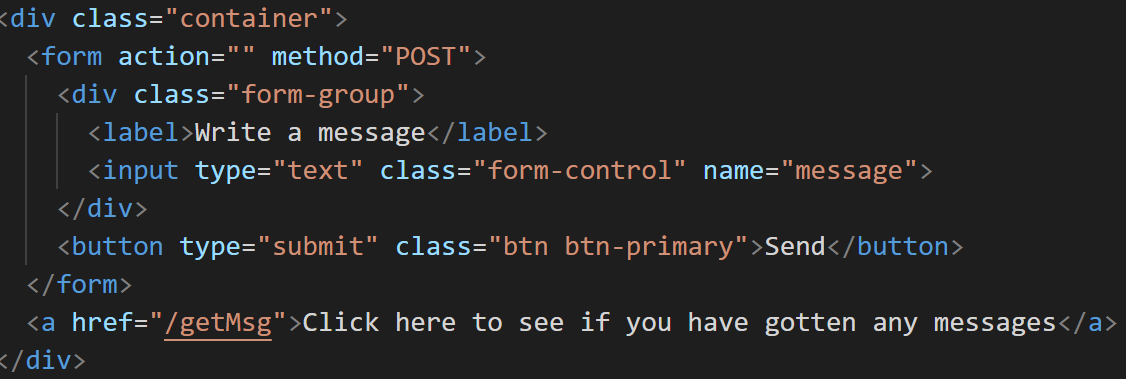
\includegraphics[width=\linewidth]{code_snippets/temp.PNG}
  \caption{The template that shows an input field to write a message and a submit button}
  \label{fig:temp}
\end{figure}

If Bob writes a message and clicks enter or submit, the message will be encrypted using SDES with the secret key from the Diffie-Hellman key exchange. As shown in Figure \ref{fig:sendMsg}, if there is some text in the message field the message gets converted into 8 bits block and encrypted. I do not hold any history of the previous messages, so if Bob writes a new message for Alice, it will overwrite the previous message.

\begin{figure}[H]
  \hspace*{-50px}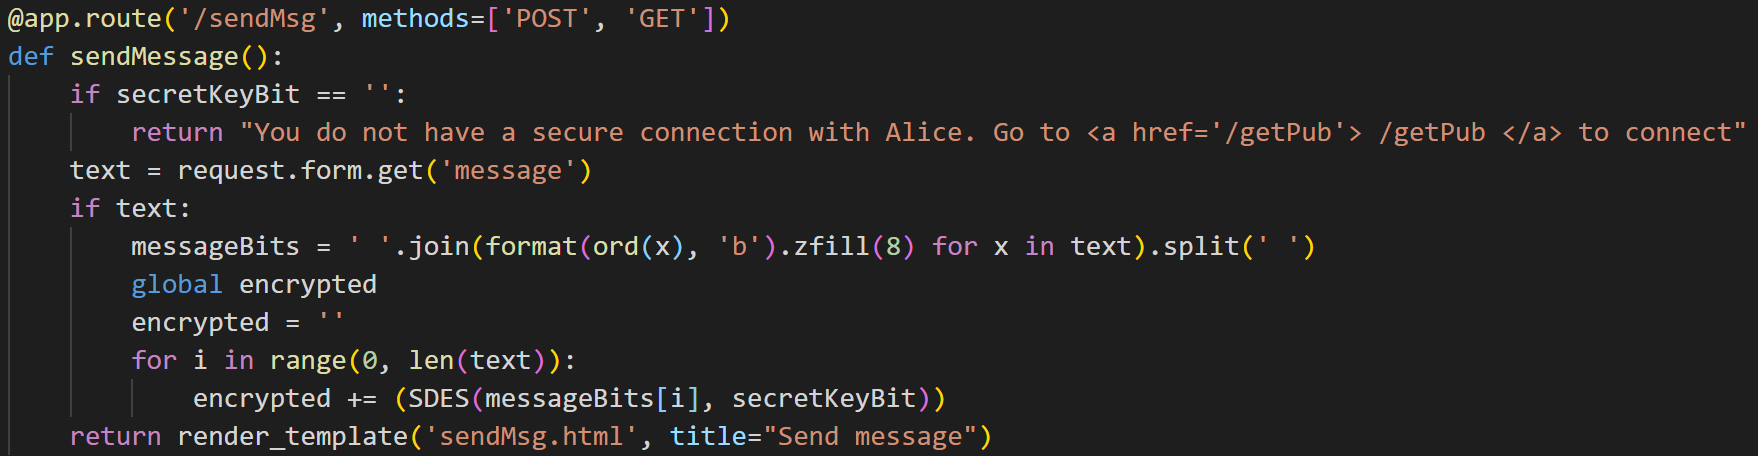
\includegraphics[width=500px]{code_snippets/sendMsg.PNG}
  \caption{If a message is sent it will be encrypted}
  \label{fig:sendMsg}
\end{figure}

When a message is submitted from Bob and it is encrypted, the cipher will be returned at /sentMsg, as shown in Figure \ref{fig:sentMsg}. That is the endpoint Alice want's to fetch to get the messages from Bob.

\begin{figure}[H]
  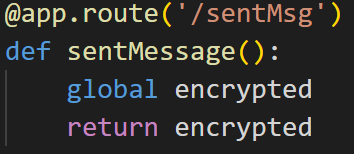
\includegraphics[width=150px]{code_snippets/sentMsg.PNG}\centering
  \caption{The fetching point for the other server to get the encrypted message}
  \label{fig:sentMsg}
\end{figure}

When Alice wants to see if there is a message from Bob, she will go to /getMsg. As for all pages, if you want to connect to the other server, you need a secure connection and if you do not have that, you will just get a message to go to /getPub. If Alice has a secure connection with Bob her server will fetch Bob's /sentMsg, as shown in Figure \ref{fig:getMsg}. The result from the fetch will be split into 8-bit blocks and decrypted using SDES and their shared secret key. If there is no message and nothing has been decrypted there will be displayed a message telling that there is no message, but if you want to send one to Bob, go to /sendMsg. If there is a message from Bob, the message will be displayed in a <h3> bracket, so that it is clear what the message is. 

\begin{figure}[H]
  \hspace*{-50px}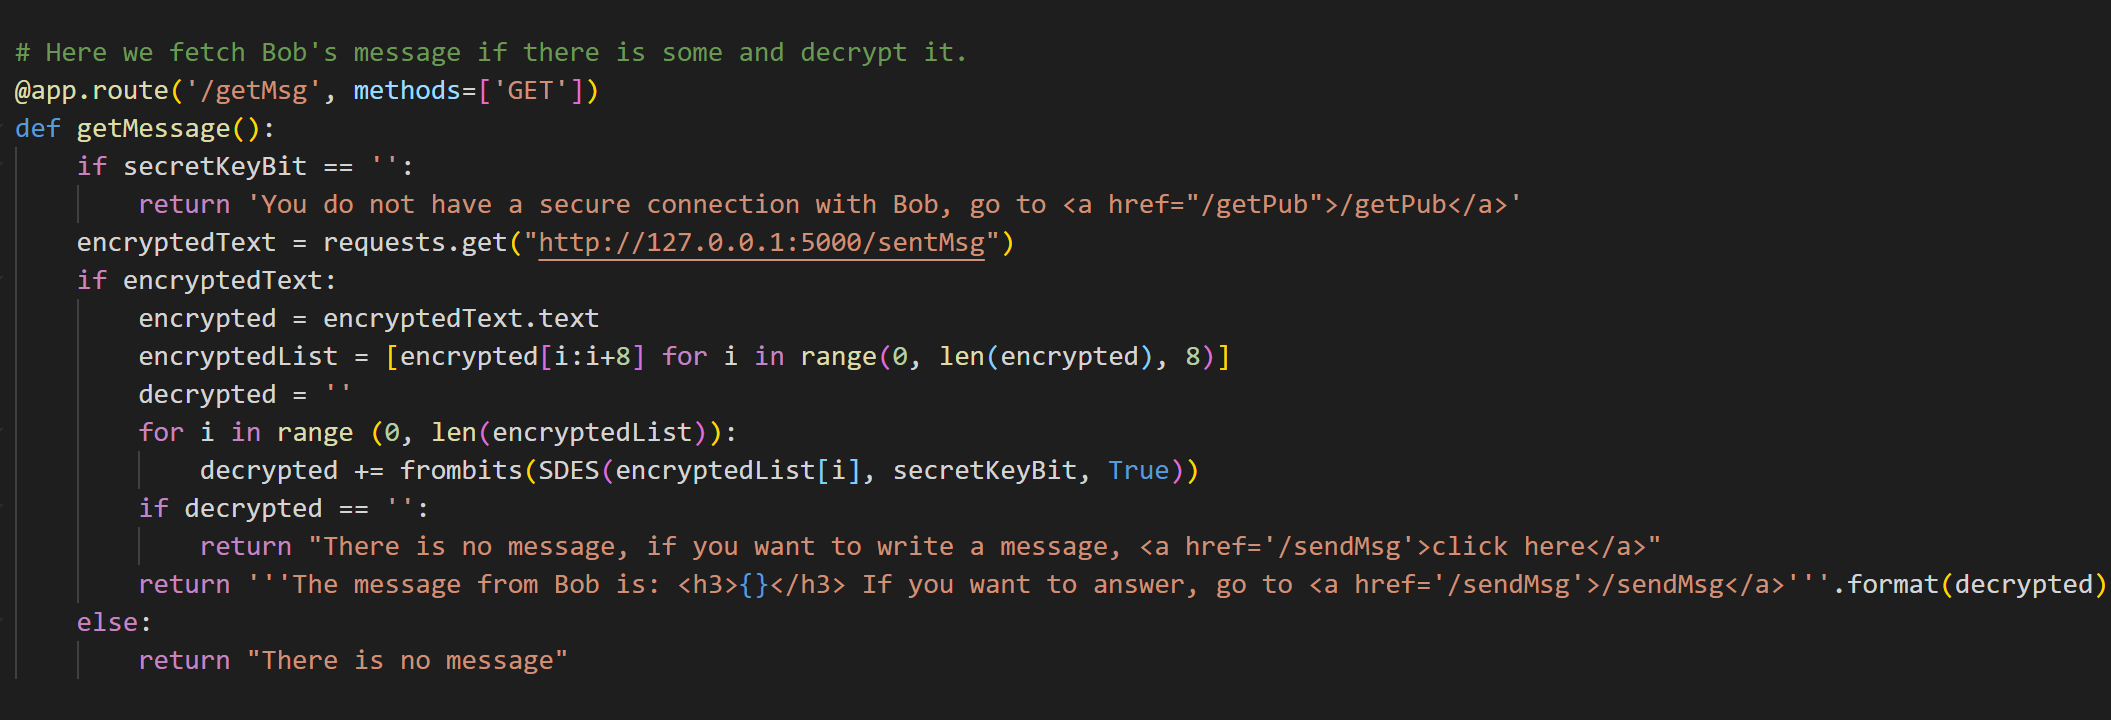
\includegraphics[width=500px]{code_snippets/getMsg.PNG}
  \caption{Will fetch and display the messages from Bob if there is any}
  \label{fig:getMsg}
\end{figure}

The code on both Alice's and Bob's side are, as said, very similar. The difference is the messages displayed and the port they are fetching from. So Alice can send messages to Bob and vice versa. If Alice has created a secure connection with Bob, she can send messages, but Bob can't get the messages before he has a secure connection as well. Without a secure connection, they cannot encrypt or decrypt the messages. 

\section*{Test results}

\subsection*{Part 1}
In Figure \ref{fig:runYN} you can see the result of the staged scenario of creating a secure connection using Diffie-Hellman key exchange and Blum Blum Shub. First, we display the information about the shared prime, the cyclic group and the generator. Then we see the private key's to Alice and Bob, followed by their public key. If the Diffie-Hellmann key exchange goes wrong the shared key won't be printed. But as you can see in the Figure, it was successful and Alice and Bob have the same shared key, as expected. You now have the option to send a predefined message or writing your own message.

\begin{figure}[H]
  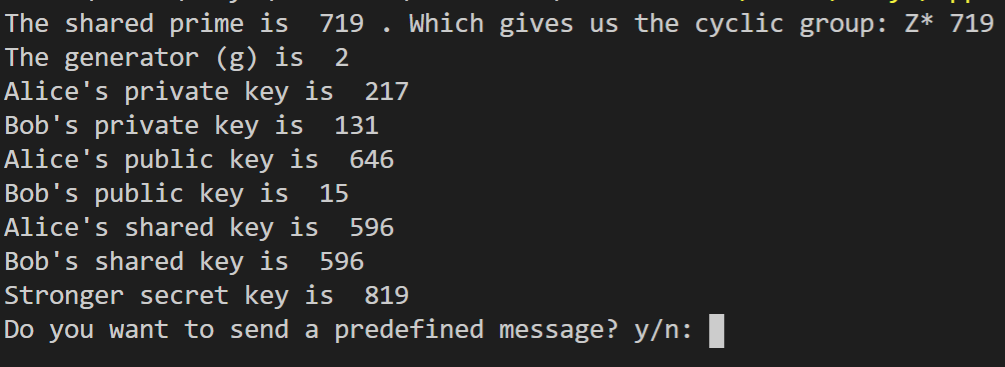
\includegraphics[width=\linewidth]{code_snippets/runYN.PNG}
  \caption{The terminal printing the public and private parameters}
  \label{fig:runYN}
\end{figure}

In Figure \ref{fig:runY} you see the result of using the predefined message \textit{this is a super secret message}. I have also printed the encrypted message in binary. The last line shows the message after being by Bob. And as you can see we got the expected result.

\begin{figure}[H]
  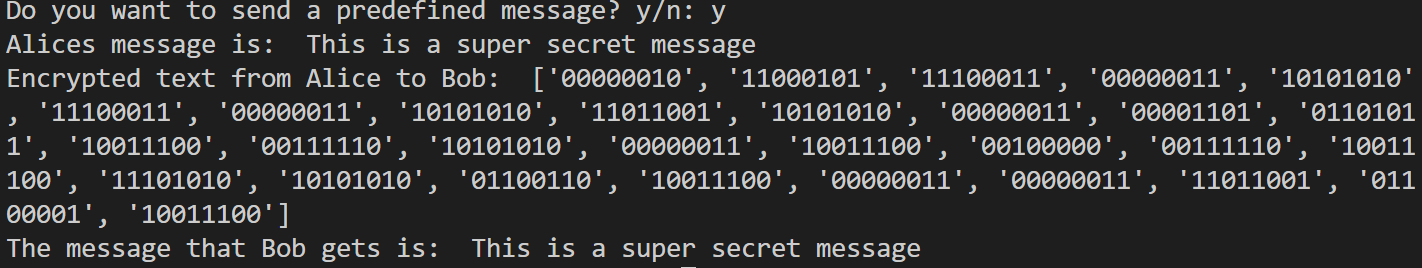
\includegraphics[width=\linewidth]{code_snippets/runY.PNG}
  \caption{The terminal printing the encryption and decryption with a predefined message}
  \label{fig:runY}
\end{figure}

I have added the opportunity to write your own message, and an example of that is shown in Figure \ref{fig:runN}. We still get the expected result.

\begin{figure}[H]
  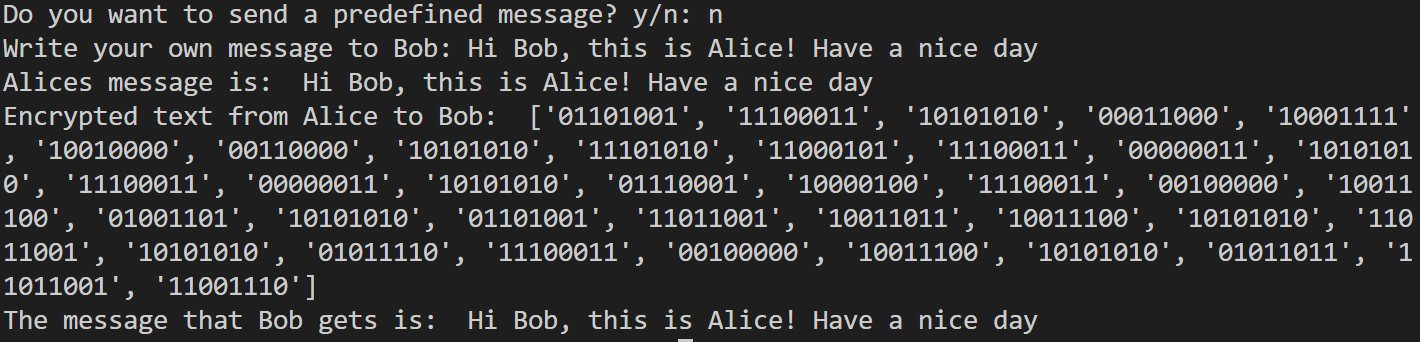
\includegraphics[width=\linewidth]{code_snippets/runN.PNG}
  \caption{The terminal printing the encryption and decryption taking in the message as input}
  \label{fig:runN}
\end{figure}


\subsection*{Part 2}
Starting up the two servers will look like shown in Figure \ref{fig:front}. The link will move you on to /getpub to do the Diffie-hellman key exchange and create a secure connection.

\begin{figure}[H]
  \hspace*{-50px}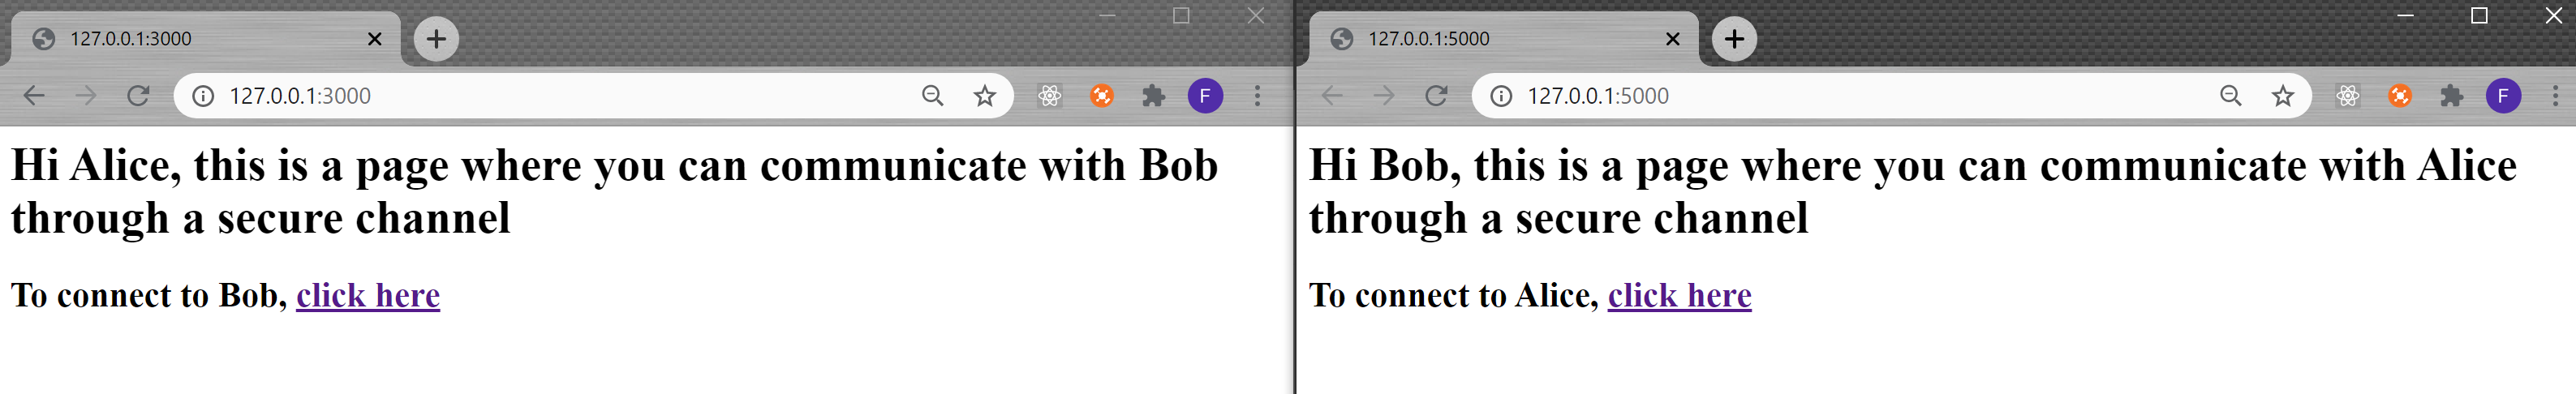
\includegraphics[width=500px]{code_snippets/front.PNG}
  \caption{The homepage}
  \label{fig:front}
\end{figure}

When you go to /getpub and get the message as shown in Figure \ref{fig:getpubpage}, it means that you successfully fetched the other parts public key and the Diffie-Hellmann key exchange went as expected. When the secure connection is established you get a link to the /sendMsg page.

\begin{figure}[H]
  \hspace*{-50px}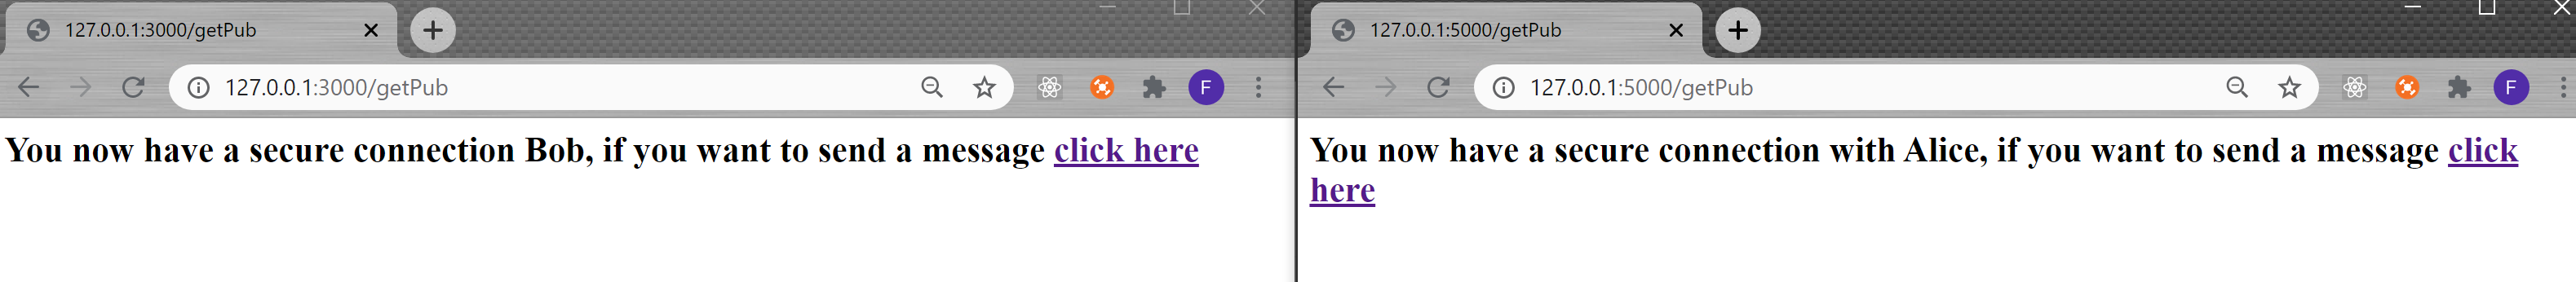
\includegraphics[width=500px]{code_snippets/getpubpage.PNG}
  \caption{The page to establish a secure connection}
  \label{fig:getpubpage}
\end{figure}

At the /sendMsg page you can write a message in the input field as shown in Figure \ref{fig:sendmsgpage}. After writing some message and clicking enter or the Send button the input field will be cleared and the message is sent. There is also a link under the input field where you can click to see if you have gotten any messages from the other server.

\begin{figure}[H]
  \hspace*{-50px}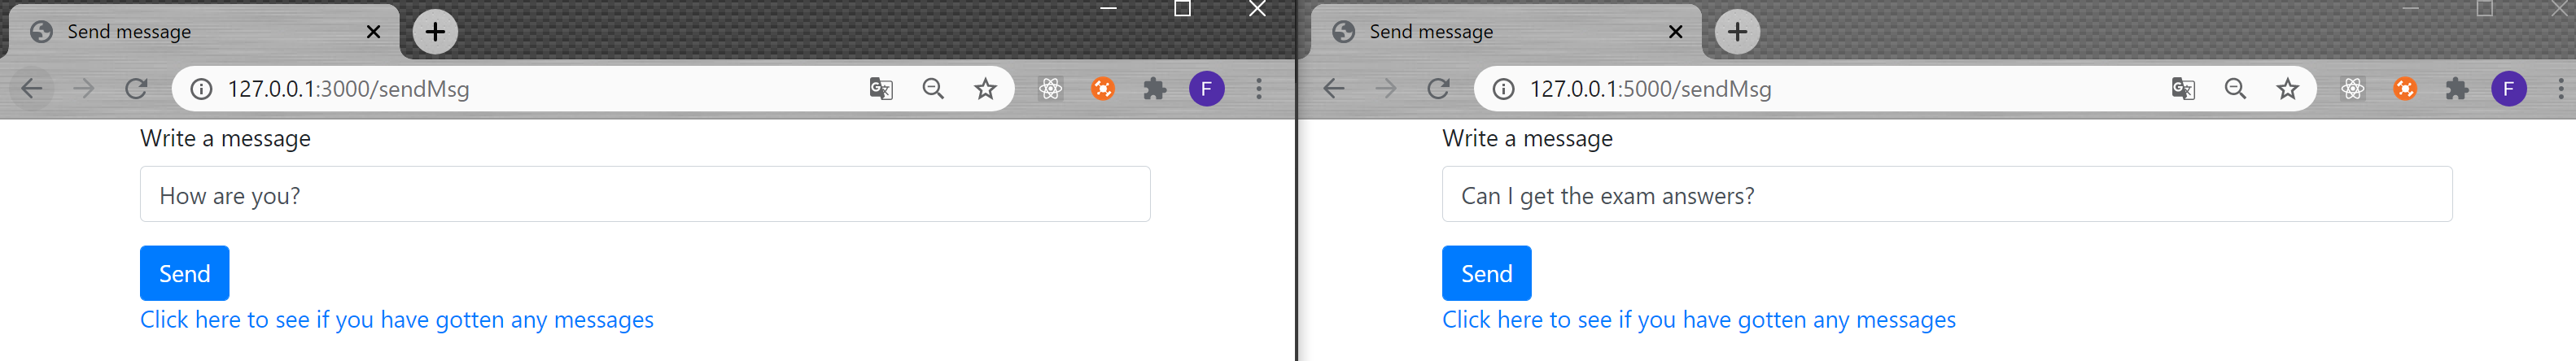
\includegraphics[width=500px]{code_snippets/sendmsgpage.PNG}
  \caption{The page where you can send messages}
  \label{fig:sendmsgpage}
\end{figure}

Figure \ref{fig:getmsg} shows how it will look if you have gotten a message. If there is no message it will be displayed "There is no message" instead. Regardless of whether it is a message or not, there will be a link to /sendMsg. 

\begin{figure}[H]
  \hspace*{-50px}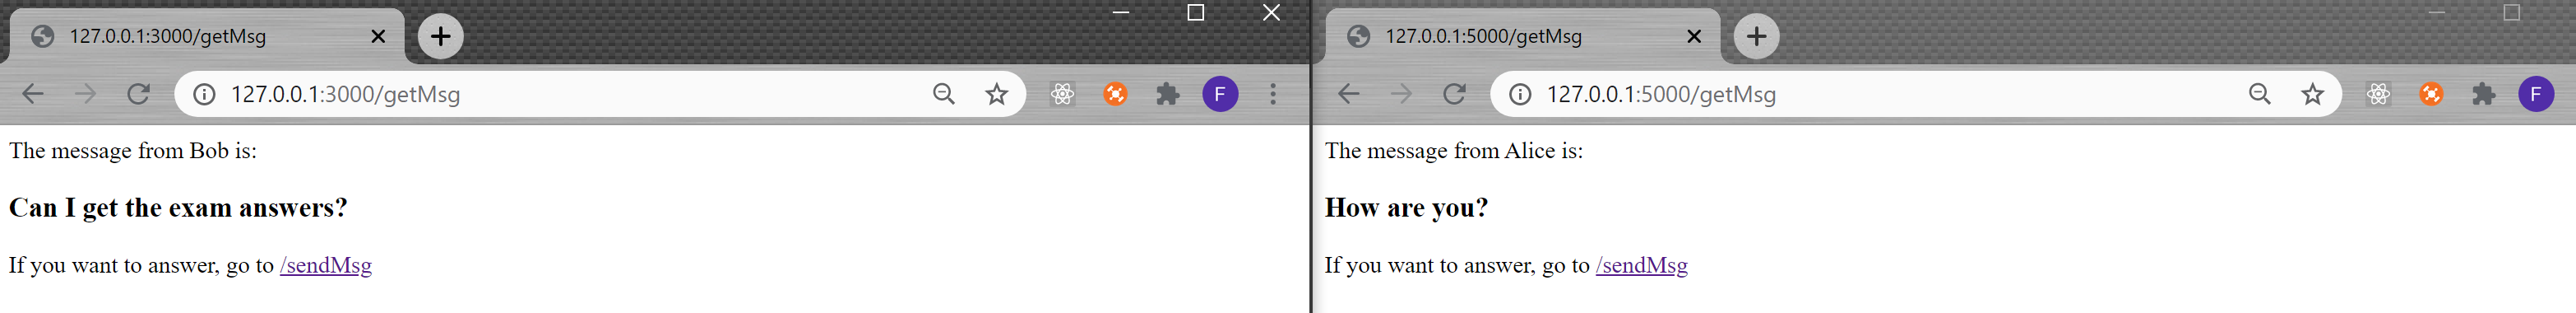
\includegraphics[width=500px]{code_snippets/getmsgpage.PNG}
  \caption{The page where you can see the message if there is one}
  \label{fig:getmsg}
\end{figure}

If you try to go to some other page than /getPub to start of with, you will get always get the message that is shown in Figure \ref{fig:notsecure}

\begin{figure}[H]
  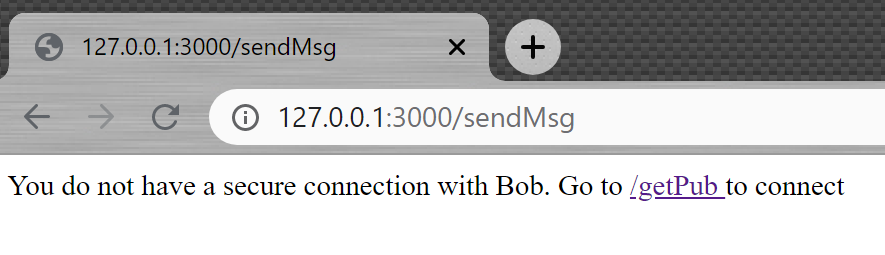
\includegraphics[width=\linewidth]{code_snippets/notsecure.PNG}
  \caption{The message shown if you have not done Diffie-Hellman key exchange by going to /getPub}
  \label{fig:notsecure}
\end{figure}

\section*{Discussion}

\subsection*{Part 1}
The first part of the assignment is to implement a secure communication scenario that included creating my own key exchange system and CSPRNG. I chose to use the Diffie-Hellman key exchange scheme, but I could have used the elliptic curve-based Diffie-Hellman scheme as well. As far as I have understood, both are used today. But elliptic curve-based Diffie-Hellman would have been cool to implement as well. But for this assignment, a normal Diffie-Hellman key exchange scheme is more than good enough. For reflection, I am actually very impressed with how the concept of modulo can be used in a so smart and simple way to generate an important security concept. When it comes to the cryptographically strong pseudo-random number generator I think using Blum Blum Shub, in this case, was a good decision. It is maybe the strongest proven random number generator. But it is also a slow algorithm, but in this case, we are not working with gigantic numbers, and therefore it is beneficial in this case.

When it comes to showing the results in the print statements, I think it is easy to follow the steps and see that everything works out as planned. I did not want to write even more details in the print statements, because the main task here was to show how it works and the results on the way. 

\subsection*{Part 2}
The second part of the assignment used the elements from part 1, but instead of staging a scenario, we did perform the steps using two servers. The servers did work as expected and performed the stages of Diffie-Hellman key exchange, Blum Blum Shub, and encrypting and decrypting messages. If I would have more time I would have done the pages prettier and maybe created a button for creating the secret key instead of an URL. But in the end, I think it works as expected and this is not a design and user experience course. Both Alice and Bob can connect and send encrypted messages and decrypt them.

\section*{Conclusion}
To conclude this assignment I will say that I have learned in-depth about the Diffie-Hellman key exchange and Blum Blum Shub and implemented them. I have also learned about other alternatives as well, even though I have not implemented them. The servers on the two different ports were created and could demonstrate how the concepts can work on a web server and I got a result where Alice and Bob could communicate to each other on a secure channel.

\begin{thebibliography}{10} 
\bibitem{BBS} A Security site,  \emph{Explaines how Blum Blum Shub works},
\url{https://www.asecuritysite.com/encryption/blum}.
\bibitem{DH} Wikipedia,  \emph{Wikipedia - Diffie-Hellman},
\url{https://en.wikipedia.org/wiki/Diffie%E2%80%93Hellman_key_exchange}.
\end{thebibliography}



\end{document}